%!TEX root = ../dissertation.tex
\begin{savequote}[75mm]
We must be prepared to accept the possibility that what we call ``the environment'' may lie, in part, within the skin of the biological organism
\qauthor{Herbert Simon (\citeyear{simon1955behavioral})}
\end{savequote}

% \chapter{Formalism}
\Chapter[Meta-level Markov decision processes]{Formalism}\label{sec:metamdp}
% \begin{flushright}
% {\large\itshape Meta-level Markov decision processes}
% \vspace{1.3\baselineskip}
% \end{flushright}

\newthought{The key insight} behind the proposed framework is that cognitive processes are solutions to sequential decision problems. Drawing on a subfield of artificial intelligence known as \emph{rational metareasoning} \citep{matheson1968economic,russell1991principles}, we formalize this insight using the framework of \emph{metalevel Markov decision processes} (metalevel MDPs; \citealp{hay2012selecting}). In this framework, a cognitive process is formalized as a sequential process of executing computational actions that update an agent's mental state. At each moment, the agent must choose whether to continue thinking, refining their mental state but accruing computational cost, or to instead stop thinking and take action. In the former case, they must additionally decide which computation to execute next (i.e., what to think about). In the latter case, they select the action that seems best given their current mental state and receive a reward associated with the external utility of that action.

% in the latter case, they select the optimal action given their current belief and receive a reward associated with the external utility of that action.

In this chapter, I provide a formal description of the framework. The formalization presented here is an adaptation of the framework proposed in \citet{hay2016principles}. I have modified the framework to better facilitate the specification of cognitive models.

% We begin by introducing Markov decision processes (MDPs). Next, we define metalevel MDPs as extensions of standard MDPs. Finally, we define a specific metalevel MDP model for multi-attribute decision-making, which we will employ in our experimental case studies.

% Below, we give a high-level and intuitive overview of the general framework and its application to multi-attribute choice, the domain we will use in our case studies. A formal treatment is provided in Appendix~\ref{metamdp}.

% We begin by describing, in intuitive terms, how the framework can be applied to model multi-attribute decision-making. Next, we will formally define metalevel MDPs. Finally, we will return to the multi-attribute decision-making case, showing how the formalism can be applied to a specific case.

\begin{figure*}
  \centering
  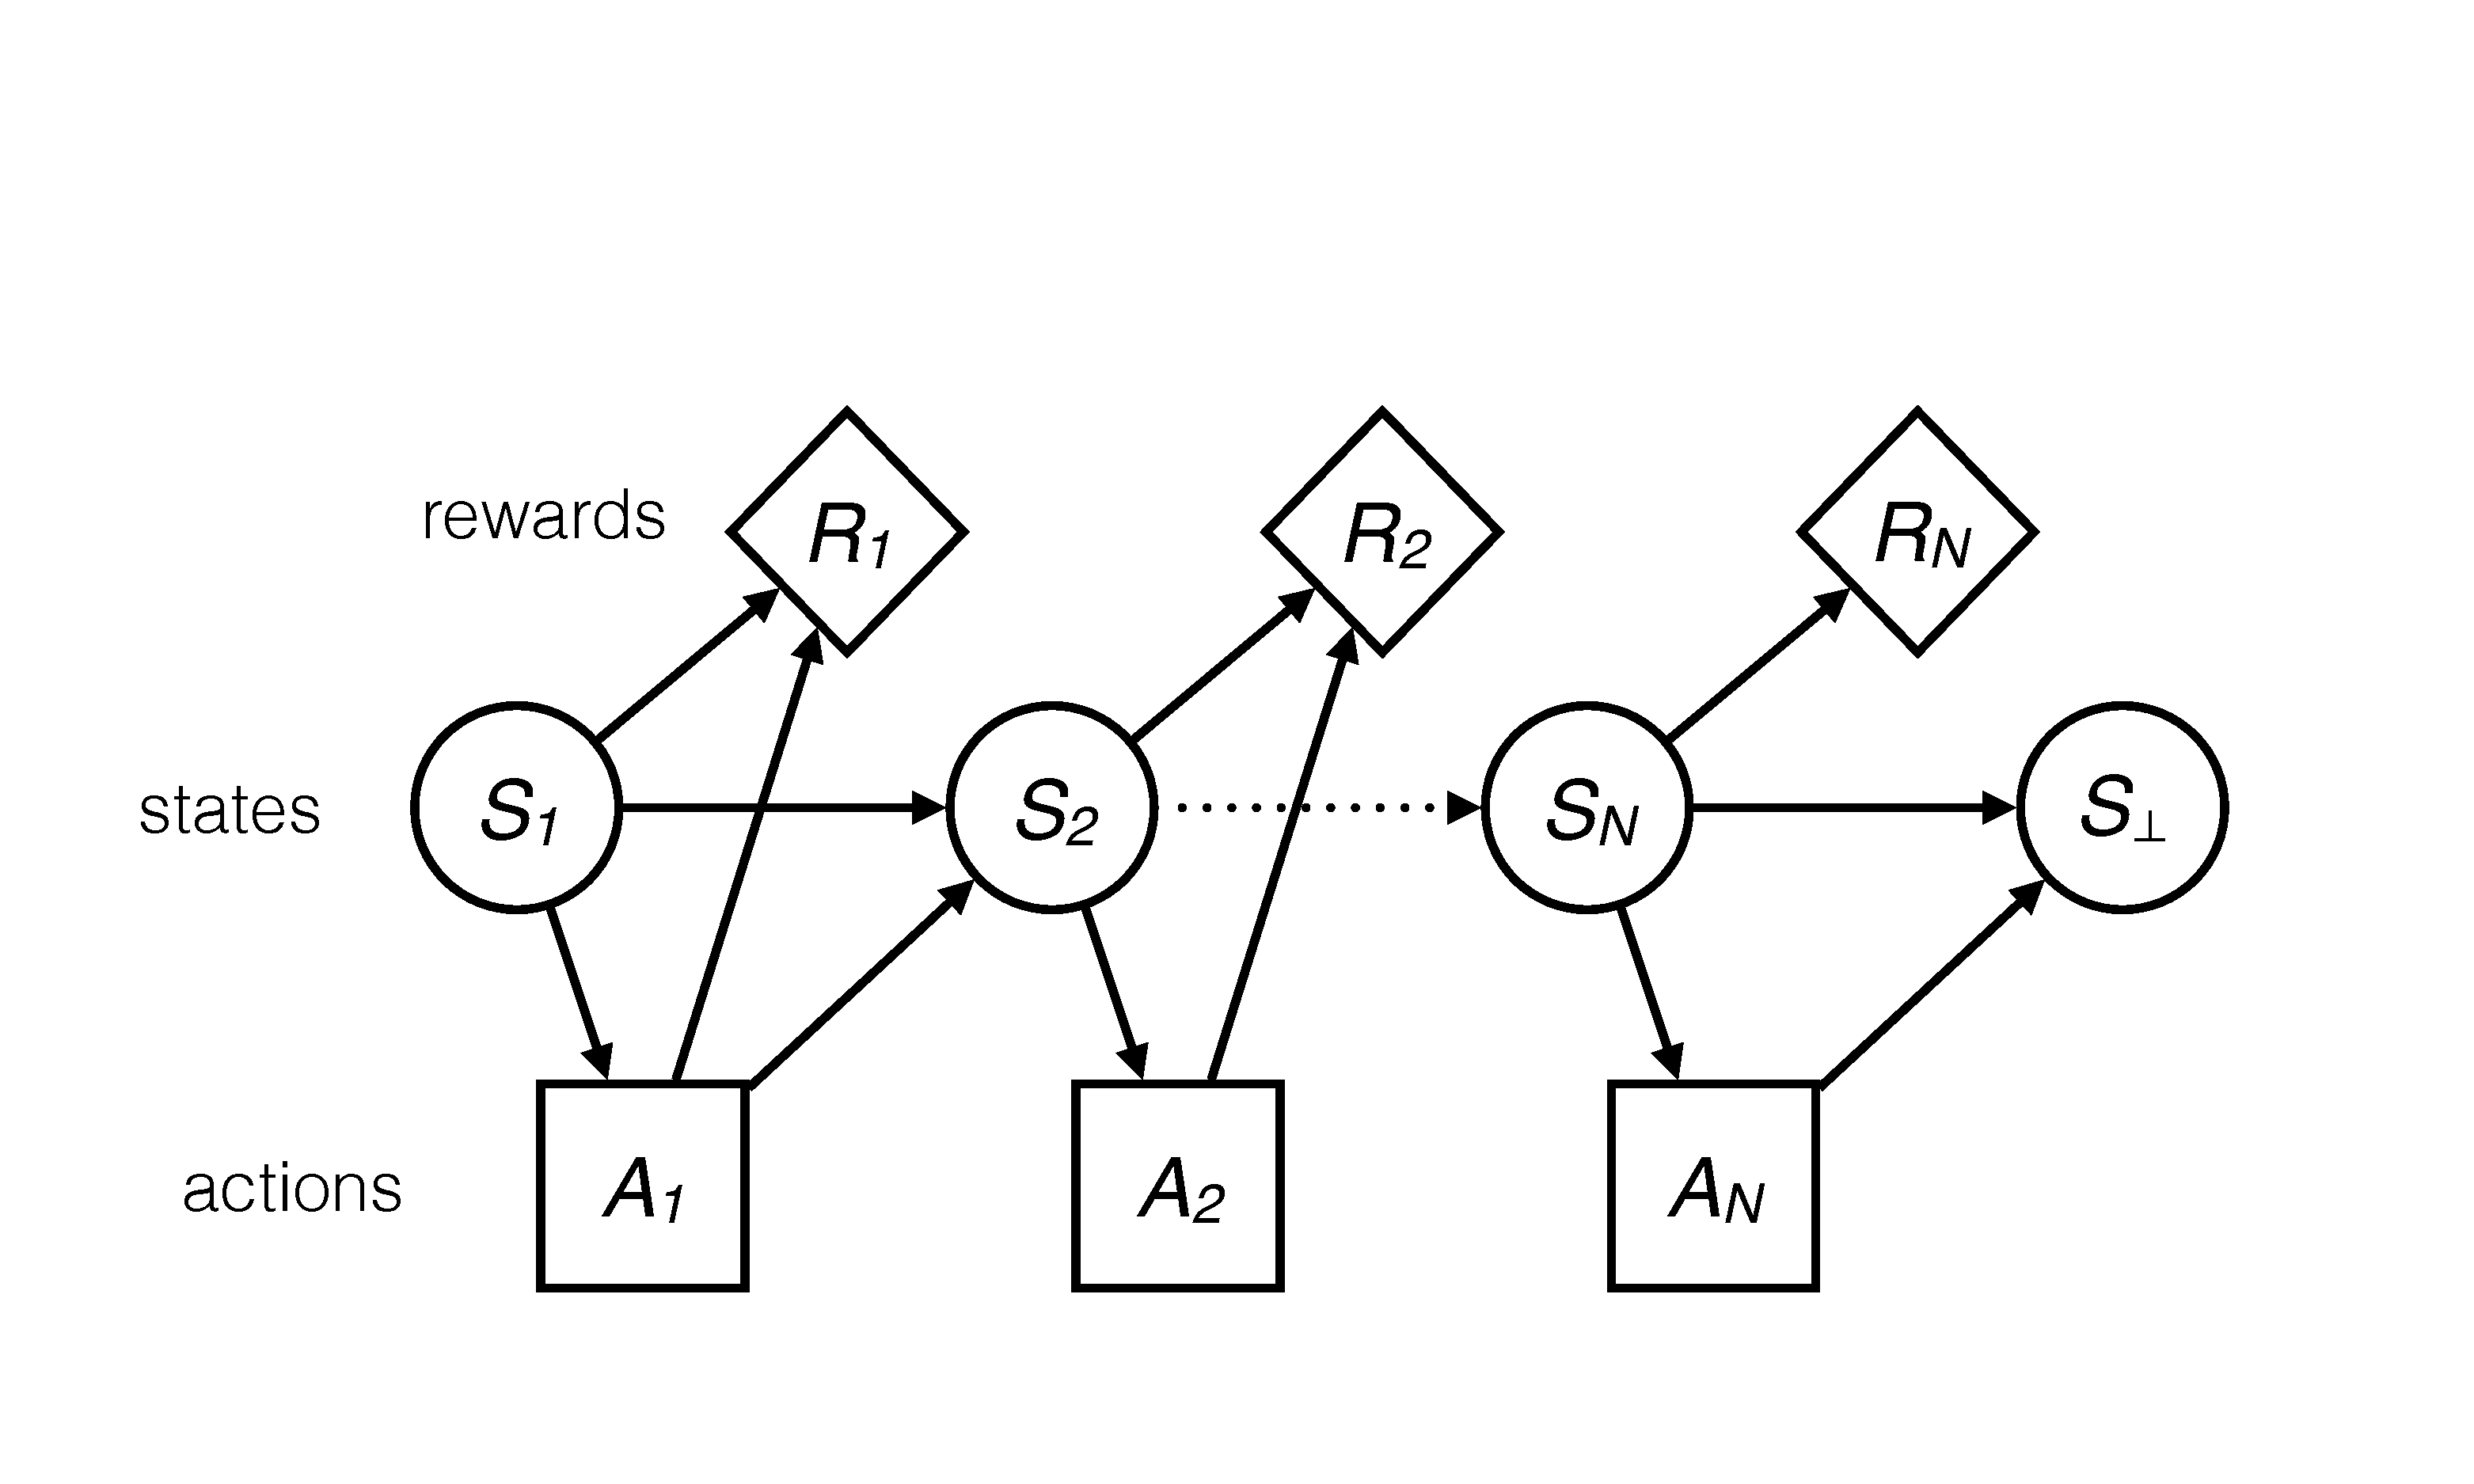
\includegraphics[width=0.8\textwidth,page=1,trim=0 100 0 200]{diagrams/metamdp.pdf}
  \caption{\captiontitle{Markov decision processes.}
    A Markov decision process (MDP) formalizes the problem of acting adaptively in a dynamic environment. The agent executes actions (squares) that change the state of the world (circles) and generate rewards (diamonds), which the agent seeks to maximize. The arrows indicate direct causality; thus, the reward and state at each time step depend only on the state and action at the previous time step, and the agent selects an action based only on the current state. The dotted arrow indicates the elided sequence of states between the first and last two.
  }
  \label{fig:mdp-diagram}
\end{figure*}


\section{Markov decision processes}\label{sec:mdps}

A metalevel Markov decision process is an extension of a standard Markov decision process (MDP), illustrated in \figref{fig:mdp-diagram}{}. Thus, I begin with a brief overview of standard MDPs. See \citet{puterman2014markov} and \citet{sutton2018reinforcement} more thorough overviews.

MDPs are the standard formalism for modeling the sequential interaction between an agent and a stochastic environment. An MDP is defined by a set of states $\S$, a set of actions $\A$, a transition function $T$, and a reward function $R$. A state $s \in \S$ specifies the relevant state of the world. An action $a \in \A$ is an action the agent can perform. The transition function $T: \S \times \A \rightarrow \Delta(\S)$\footnotemark{} encodes the dynamics of the world as a distribution of possible future states for each possible previous state and action. Finally, the reward function $R: \S \times \A \rightarrow \R $ specifies the expected\footnote{%
  One could equally well specify a stochastic reward function $R: \S \times \A \rightarrow \Delta(\R)$. Because the optimal policy only depends on the expected reward, we do not consider this case here. However, a stochastic reward function would affect the performance of a learning algorithm; this could easily be integrated into the framework.
} reward or utility for executing a given action in a given state. We additionally assume an initial state $s_1$ that the environment is initialized in and a set of terminal states $\S_\bot$ such that the episode ends when the agent reaches one of those states. An \emph{episode} describes one interaction between the agent and the environment (beginning in the initial state and ending in a terminal state).

\footnotetext{%
  $\Delta(\S)$ denotes the set of all distributions over the set $\S$. Note that this definition is equivalent to defining the transition function as a probability mass function (i.e., $T: \S \times \A \times \S \rightarrow [0, 1])$. I will use $T(s' \mid s, a)$ to denote the probability of transitioning to state $s'$ when executing action $a$ in state $s$.
  % However, defining transition functions in this way is often highly unintuitive. We will thus instead define transition functions as generative probabilistic models. This notation reflects that choice.
}


\subsection{Optimal policies and value functions}

The solution to an MDP is a policy $\pi: \S \rightarrow \Delta(\A)$ that selects which action to perform next given the current state. That is, $a_t \sim \pi(s_t)$. The goal is to find a policy that maximizes the expected cumulative reward attained, that is, the \emph{return}. The optimal policy is thus defined,
\begin{equation}\label{eq:optimal-policy}
  \pi^* = \argmax_\pi \expect{
    \sum_{t=1}^{\tmax} R(s_t, a_t)
  }{
   a_t \sim \pi(s_t)
  },
\end{equation}
where $\tmax$ is the timepoint at which the episode terminates (when $s_{t+1} \in \S_\bot$). Note that the expectation implicitly conditions on the transition function, i.e., $s_{t+1} \sim T(s_t, a_t)$.

How can we identify such a policy? This question is the subject of a huge field of research in artificial intelligence, and countless methods have been developed. Many of these methods draw on the concept of a \emph{value function}. The \emph{state} value function (or just ``value function'') is defined as
%
\begin{equation}\label{eq:state-value}
  V^\pi(s) = \expect{
    \sum_{t=1}^{\tmax} R(s_t, a_t)
  }{
   s_1 = s,\ a_t \sim \pi(s_t)
  }.
\end{equation}
%
It specifies the expected total reward one will receive if one begins in state $s$ and selects actions according to the policy $\pi$. Similarly, the \emph{action} value function (or ``state-action value function'') is defined as
%
\begin{equation}\label{eq:action-value}
  Q^\pi(s, a) = \expect{
    \sum_{t=1}^{\tmax} R(s_t, a_t)
  }{
   s_1 = s,\ a_1 = a,\ a_{t \neq 1} \sim \pi(s_t)
  }.
\end{equation}
%
The action value function just like the state value function except that it also specifies the first action to be taken. 

The value functions for the optimal policy are called the optimal value functions. They can be defined simply $V^* = V^{\pi^*}$ and $Q^* = Q^{\pi^*}$. By combining Equations~\ref{eq:state-value} and~\ref{eq:action-value} with Equation~\ref{eq:optimal-policy}, we can see that the optimal value functions specify the maximal expected reward one could expect to gain beginning with a given state (and action) under any policy,
\begin{equation}
  \begin{aligned}
  V^*(s) &= \max_\pi \expect{
    \sum_{t=1}^{\tmax} R(s_t, a_t)
  }{
   s_1 = s,\ a_t \sim \pi(s_t)
  } \\
  Q^*(s, a) &= \max_\pi \expect{
    \sum_{t=1}^{\tmax} R(s_t, a_t)
  }{
   s_1 = s,\ a_1 = a,\ a_{t \neq 1} \sim \pi(s_t)
  }
  \end{aligned}
\end{equation}

Putting aside for now the problem of identifying these functions, the optimal policy can be defined as simply
%
\begin{equation}\label{eq:argmaxQ}
  \pi^*(s) = \Uniform\left(\argmax_a Q^*(s, a)\right).
\end{equation}
%
That is, the optimal policy selects the action that produces the greatest expected long-term reward, breaking ties randomly.\footnote{%
  To be more precise, Equation~\ref{eq:argmaxQ} defines the \emph{maximum entropy} optimal policy, that is, the optimal policy whose action distributions are maximally random. For simplicity, I will refer to the maximum entropy optimal policy as simply ``the'' optimal policy.
} When modeling human data, one typically assumes that this maximization is performed imperfectly. In particular, we will assume that actions are drawn according to a softmax (or Boltzmann distribution),
%
\begin{equation}\label{eq:softoptimal}
  \pi(a \mid s) \propto \expp{\beta \cdot Q^*(s, a)}
\end{equation}
% \displaystyle\sum_{a'} \expp{\beta \cdot Q^*(s, a')}
%
where the inverse-temperature parameter $\beta$ controls how well the policy maximizes, behaving completely randomly when $\beta = 0$ and approaching the optimal policy as $\beta \rightarrow \infty$.

This concludes our brief overview of MDPs. We are now ready to describe metalevel MDPs.

% An important property of MDPs is that there is at least one deterministic \emph{optimal policy}; that is, there is a mapping from states to actions that, when followed, will produce the maximum possible return. 

\begin{figure*}
  \centering
  \includegraphics[width=0.8\textwidth,page=2,trim=0 100 0 50]{diagrams/metamdp.pdf}
  % 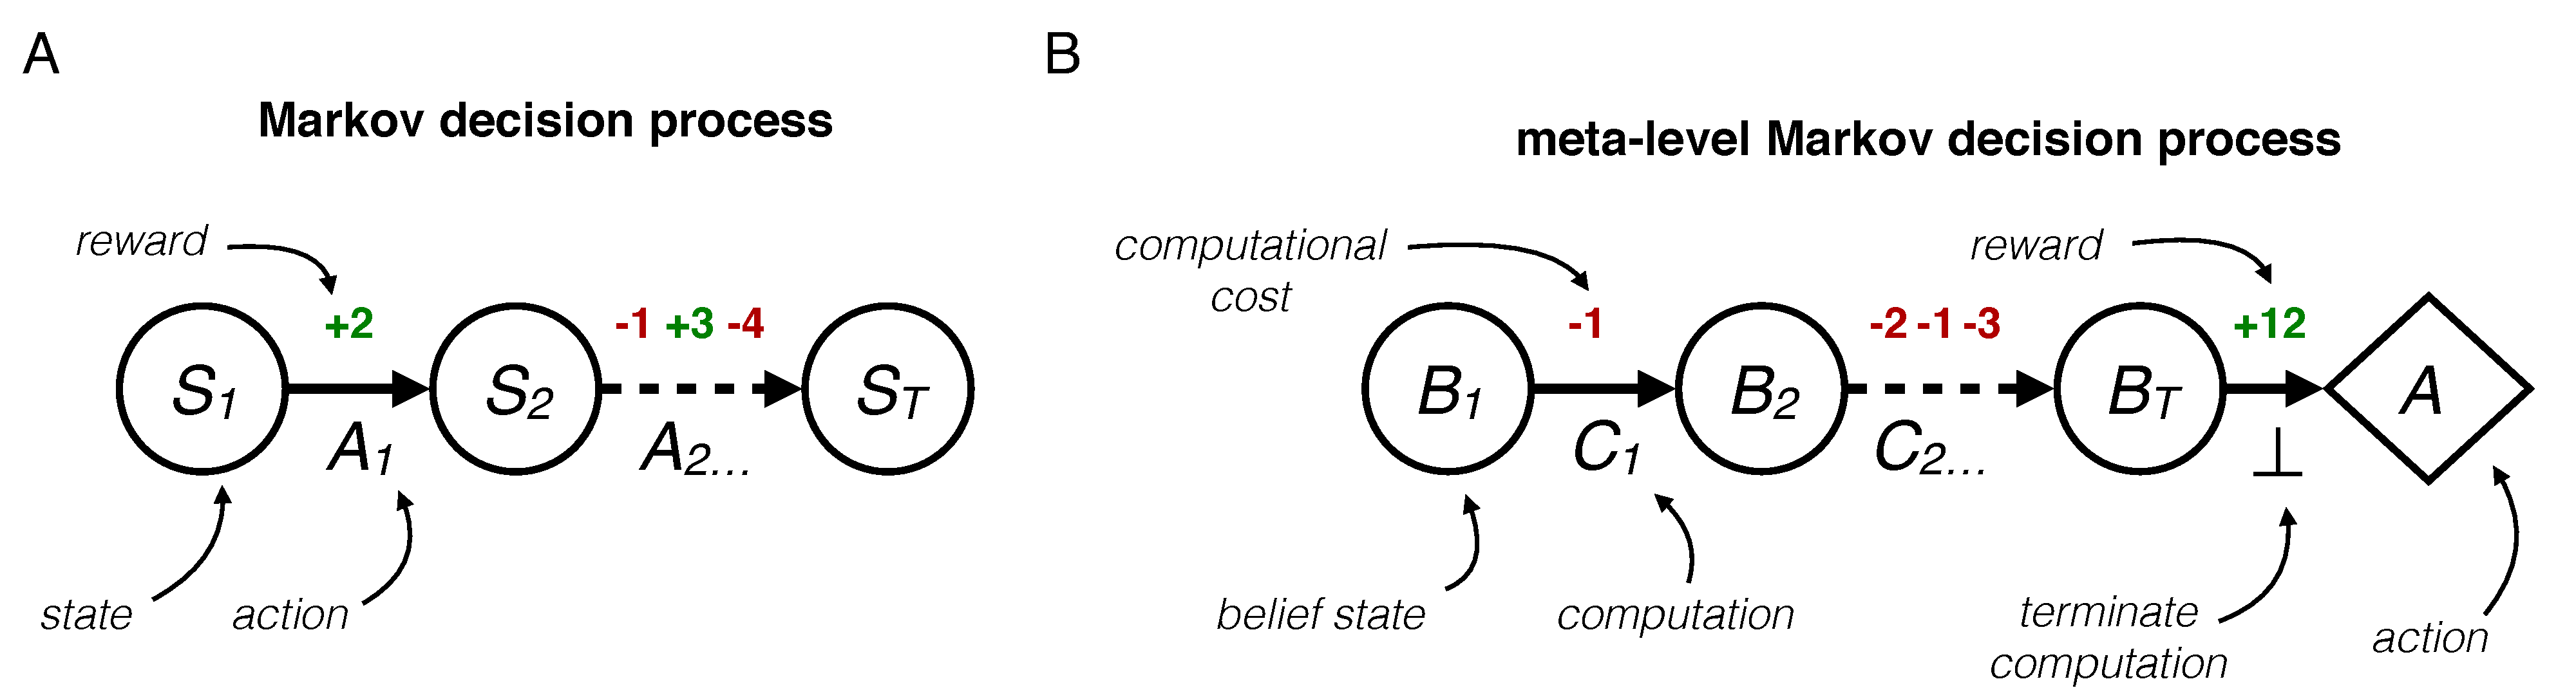
\includegraphics[width=\textwidth]{figs/metamdp.pdf}
  \caption{\captiontitle{Metalevel Markov decision processes}.
    A metalevel MDP formalizes the problem of thinking efficiently within one's own internal mental environment. The agent executes computations that update their mental state and incur cognitive cost. When the agent executes the termination operation $\bot$, they take an action in the external environment and receive an external reward. The elements that capture the external environment are indicated in blue. These formally distinguish metalevel MDPs from standard MDPs.
  }
  \label{fig:metamdp-diagram}
\end{figure*}



\section{Metalevel Markov decision processes}\label{sec:metalevel-mdps}

% The concept is thus very similar to \emph{elementary information processes} \citep{chase1978elementary,simon1979information,posner1982information,payne1988adaptive}. 

Meta-level Markov decision processes (metalevel MDPs) extend the standard MDP formalism to model the sequential decision problem posed by resource-bounded computation \citep{hay2012selecting}. Like a standard MDP, a metalevel MDP is defined by sets of states and actions, and transition and reward functions. However, as illustrated in \figref{fig:metamdp-diagram}{}, the states corresponded to mental states, and the actions correspond to computations (cognitive operations). The metalevel transition function describes how computations update mental states, and the metalevel reward function captures both the internal costs (e.g., time) and external benefits (e.g., better decisions) of computation.

Formally, we define a metalevel MDP by a set of mental states $\M$, a set of computations $\C$, a transition function $T$, and a reward function $R$. These four components are analogous to the states, actions, transition function, and reward function in a standard MDP. We additionally define a set of world states $\W$, upon which the transition and reward functions depend. This is the only formal distinction between a metalevel MDP and a standard MDP. However, as I discuss in Section~\ref{sec:metamdp-marginalized}, we can sometimes convert metalevel MDPs into equivalent MDPs by marginalizing over the world state.\footnote{%
  This is similar to the \emph{belief MDP} transformation of a partially observable MDP (POMDP; \citealp{kaelbling1998planningb}). see Section~\ref{sec:pomdp} for additional discussion on the relation between metalevel MDPs and POMDPs.
} I now describe the five components of a metalevel MDP in more detail.

% We are now ready to formally specify the components of a metalevel MDP. A metalevel MDP is defined by a tuple $(\W, \M, \C, T, R)$ specifying the set of world states, the set of mental states, the set of computations, and the transition and reward functions. We describe each of these components in turn.


To make things concrete, we will use a simple running example based on the tallying heuristic for deciding between two possible actions \citep{gigerenzer2011heuristic}. We will consider applying this heuristic to the decision of which car to purchase. To follow this heuristic, we consider a sequence of ``cues'' that might discriminate between the options, marking which car each cue favors (which has better gas mileage? which is more comfortable? etc...). As we go, we simply count up how many cues have favored each car. Then, after considering some number of cues, we pick the car that is favored by more cues. But how many cues should we consider? \citeauthor{gigerenzer2011heuristic} propose considering a fixed number of cues (and, in the case of a tie, considering more cues until one car has more in its favor). Is this the best version of tallying we could use? To answer this question, we can define tallying as a metalevel MDP.

A well-documented and (hopefully) beginner-friendly Julia implementation of the tallying metalevel MDP can be found at \url{https://github.com/fredcallaway/metamdp-example}.

\subsection{World states}
A world state $w \in \W$ captures the state of the world that is relevant to the agent's current task. Importantly, the agent does not have direct access to the world state, but must infer it from the outcome of computations they perform. Formally, the world state includes any information that is not known to the agent, but affects either the reward or transition functions. In the tallying example, the world state specifies the ratio of cues that favors one car vs. the other; thus, $\W\tally = [0, 1]$. 

% One might be tempted to specify the world state as simply a binary variable indicating which car is better. However, with that definition, we could not specify the probability of drawing a cue in favor of each car in the transition function.

% For example, in a decision-making task, the world state might define the utility of the various actions available to the agent (as in Chapter~\ref{sec:attention}). In a memory task, the world state might correspond to the strength of the memory that the agent is trying to recall (Chapter~\ref{sec:memory}). 

\subsection{Mental states}

% \todo{maybe instead of m(w), use p_m(w)}
A mental state $m \in \M$ captures the agent's internal state, as relevant to the task at hand. The interpretation of a mental state can vary from model to model. In some cases, it will correspond to a belief, or a representation of the world, but it can also capture arbitrary variables in a cognitive model. In the tallying example, the mental state specifies the number of cues one has considered that favor each option. Formally, we define each $m \in \M\tally$ as a tuple $(x, y)$, where $x$ is the number of cues favoring car X and $y$ is the number of cues specifying car Y.

% The interpretation of a mental state can vary from model to model. In some cases, they will correspond to \emph{beliefs}, that is, posterior distribution over the world state. For example, in Chapter~\ref{sec:attention}, a mental state will correspond to a posterior distribution over the utilities of the items in a choice set. More generally, mental states may correspond to \emph{representations} of the world or task. This interpretation is quite natural in Chapter~\ref{sec:planning}, where mental states correspond to partially constructed decision trees. Most generally, the mental state can capture arbitrary variables in a cognitive model. For example, in Chapter~\ref{sec:memory}, the mental state specifies the activation level of a memory. 

Analogously to standard MDPs, we additionally specify an initial mental state, $m_1$. This is the mental state the agent has at the beginning of each task instance. In the tallying example, the initial mental state is defined $m_1 = (0, 0)$. Additionally, all metalevel MDPs have a single terminal state $m_\bot$, which is only entered when computation is terminated (as described below).

\subsection{Computations}
A computational operation $c \in \C$ is a primitive operation afforded by the agent's cognitive architecture. Formally, it is a metalevel action that changes the mental state in much the same way as an external action might change the world state. In a metalevel MDP model, all cognition can be broken down into a sequence of these computations, but the model makes no attempt to explain how those basic operations are themselves implemented. The concept is thus very similar to \emph{elementary information processes} \citep{chase1978elementary,simon1979information,posner1982information,payne1988adaptive}. In the tallying example, there is a single computation, which corresponds to considering another cue.

All metalevel MDPs include a special computation, the termination operation $\bot$, which indicates that computation should be terminated. Upon termination, the agent performs an external action, specifically the action that has maximal expected utility given the current mental state. Thus, the most fundamental metalevel problem---how long to compute---is captured by the decision about when to execute $\bot$. In the tallying example, executing $\bot$ corresponds to purchasing the car that is favored by more cues (choosing randomly in the case of a tie.)

\subsection{Transition function}
The transition function $T: \M \times \C \times \W \rightarrow \Delta(\M)$ describes how computation updates mental states. Formally, $T(m, c, w)$ is a distribution of possible new mental states that would result from performing a computation $c$ in mental state $m$ when the true state of the world is $w$. At each time step, the next mental state is sampled from this distribution:
\begin{equation}\label{eq:transition}
m_{t+1} \sim T(m_t, c_t, w).
\end{equation}
Terminating computation (executing $\bot$) always transitions to the terminal state, $m_\bot$:
%
\begin{equation}
  T(m, \bot, w) = \Uniform(\{m_\bot\})
\end{equation}

In the tallying example, the transition function specifies the probability that each cue count will be incremented when one considers another cue:
\begin{equation}\label{eq:tally-transition}
  T\tally(m_t, c_t, w) = \begin{cases}
    (x_t + 1, y_t) &\text{with probability } w  \\
    (x_t, y_t + 1) &\text{with probability } 1-w,
  \end{cases}
\end{equation}
where $m_t = (x_t, y_t)$.

\subsection{Reward function}
The metalevel reward function $R: \M \times \C \times \W \rightarrow \R$ describes both the costs and benefits of computation. It is defined in terms of three components: a cost function that specifies the cost of executing each computation, an action policy $\pi\act$ that selects an action to take given a mental state, and a utility function $U$ that specifies the utility of each possible action in each world state.

The cost of computation is captured in the reward for non-terminal operations:
%
\begin{equation}
R(m, c, w) = -\cost(m, c) \text{ for } c \neq \bot.
\end{equation}
%
We assume that the cost of a computation can depend on the current mental state but not on the state of the world. The cost of computation may include multiple factors. At a minimum, it captures the opportunity cost of the time spent executing the computation (rather than taking actions in the world). The simplest choice is to assume a constant cost for each computation executed. This is a natural choice for the tallying example, with total cost proportional to the number of cues considered.

The benefits of computation are captured by the reward for the termination operation, $R(m, \bot, w)$. Intuitively, the benefit of computation is that it allows one to take better actions in the world. Formally, the reward for termination is defined as the utility of the external action that the agent would execute given the current mental state,
%
\begin{equation}\label{eq:term-reward}
  R(m, \bot, w) = \Uterm
  % R(m, \bot, w) = \expectunder{U\left(w, a\right)}{a \sim \pi\act(m)},
\end{equation}
%
where $U(w, a)$ specifies the utility of executing action $a$ in the world state $w$ and $\pi\act$ is the \emph{action selection policy}, which chooses an action to take based on the current mental state. To simplify notation, I will assume that $\pi\act$ selects an action deterministically, but it can also return a distribution over actions. This policy should be very simple. That is, the mental state should contain sufficient information to choose an action without much additional computation.

In the tallying example, $\pi\act$ deterministically selects the car with more favorable cues, selecting randomly otherwise. Specifying $U$ is less straightforward. For simplicity, we assume that the utility derived from car X is proportional to the ratio of cues favoring X. This results in
\begin{equation}
  U\tally(w, a) = \begin{cases}
    w &\text{if } a = \mathrm{X} \\
    1-w &\text{if } a = \mathrm{Y}.
  \end{cases}
\end{equation}
Substituting our definitions of $U$ and $\pi\act$ into Equation~\ref{eq:term-reward} yields:
\begin{equation}
  R\tally(m, \bot, w) = \begin{cases}
    w &\text{if } x_t > y_t \\
    1-w &\text{if } x_t < y_t \\
    \nicefrac{1}{2} &\text{if } x_t = y_t
  \end{cases}
\end{equation}
% $R(m, \bot, w)$ for the tallying example, we will assume that 
where the $\nicefrac{1}{2}$ comes from taking the average of $w$ and $1 - w$.

Equation~\ref{eq:term-reward} may appear to constrain us to simple one-shot decision-making tasks, such as the ones tallying is intended for. However, it is not as restrictive as it first appears. For example, in Chapter~\ref{sec:memory}, we model a memory recall task by assuming that $\pi\act$ can only perform the ``recall'' action when the activation of a memory exceeds a threshold. In Chapter~\ref{sec:planning}, we model a planning task by defining $a$ abstractly, as a sequence of concrete actions (or more generally, an \emph{option}; \citealp{sutton1999mdps}).\footnote{
  This does require that all computation is executed before any external action is performed, but this constraint does not reduce performance in deterministic environments. See Section~\ref{sec:interleaved} for a discussion of the problem of interleaved computation and action.
} 

\begin{figure}[tb!]
  \centering
  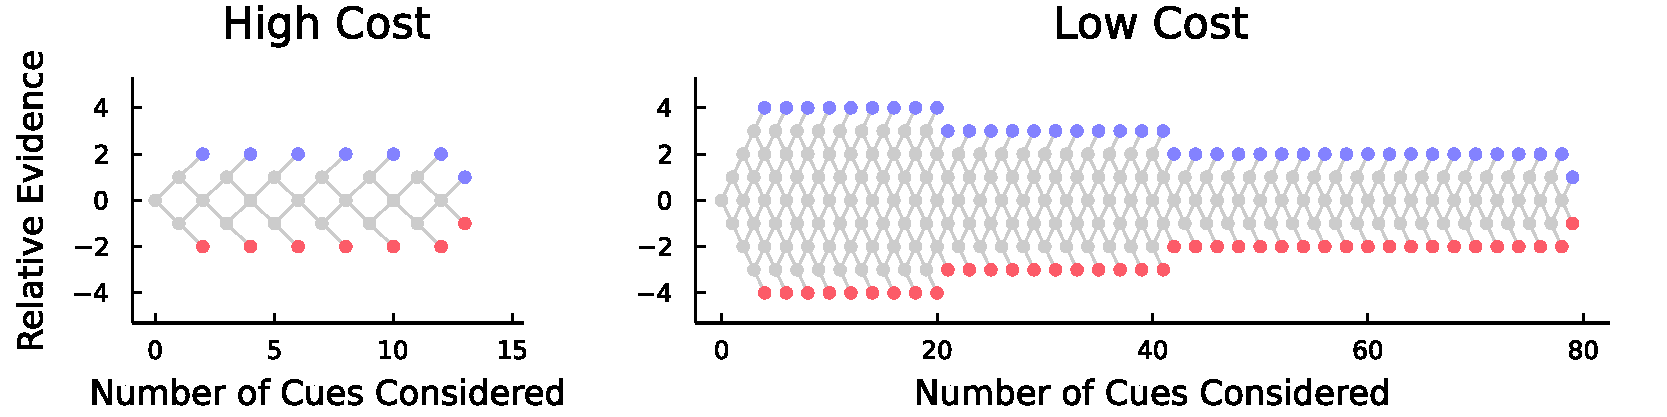
\includegraphics[width=\textwidth]{figs/policies.pdf}
  \caption{\captiontitle{Optimal policies for the tallying metalevel MDP.} 
    The policy is illustrated as a graph, where each node represents a mental state. States in which the optimal policy continues computing are gray, and states in which the optimal policy terminates are in blue and red, corresponding to the two possible external actions. The two panels show the optimal policy under different levels of computational cost (0.01 and 0.002, in units defined by the maximal action utility of 1). The code that generated this figure can be found at \url{https://github.com/fredcallaway/metamdp-example}.
  }
  \label{fig:tally-policies}
\end{figure}

\section{Metalevel policies}\label{sec:metamdp-policy}

If a metalevel MDP defines the problem a cognitive process must solve, a metalevel policy defines the solution. It is a strategy for selecting which cognitive operation to execute next given the current mental state. Formally, the metalevel policy, $\pi: \M \rightarrow \Delta(\C)$, is a mapping from beliefs to distributions over computations. At each time step, the next computation is drawn from this distribution, $c_t \sim \pi(m_t)$.

How should we determine this policy? The classical cognitive modeling approach is to specify a plausible strategy, perhaps motivated by aspects of human behavior. In Chapter~\ref{sec:planning}, we show how classical heuristics for decision-tree search can be naturally modeled as policies in a metalevel MDP. However, in the resource-rational approach pursued here, we take a different approach. Specifically, we are interested in the \emph{optimal policy} for the metalevel MDP. Paralleling Equation~\ref{eq:optimal-policy}, the optimal metalevel policy is defined as
%
\begin{equation}\label{eq:optimal-meta-policy}
  \pi^* = \argmax_\pi \expect{
    \sum_{t=1}^{\tmax} R(m_t, c_t, w)
  }{
    c_t \sim \pi(m_t)
  }.
\end{equation}
That is, it maximizes the expected return. In a metalevel MDP the return can be broken down into two components capturing the costs and benefits of computation,
\begin{equation}\label{eq:optimal-meta-policy-expanded}
  \pi^* = \argmax_\pi \expect{
    \Uterm[m_N] -
      \sum_{t=1}^{\tmax-1} \cost(m_t, c_t)
  }{
    c_t \sim \pi(m_t)
  }.
\end{equation}
This is the definition of optimal sequential cognitive processes given in Equation~\ref{eq:intro-master}.\footnote{%
  Note that the expectation implicitly depends on the transition function, which was explicit in Equation~\ref{eq:intro-master}, as well as the initial mental state $m_1$ and the set of possible computations.
} It emphasizes that the optimal policy is the cognitive strategy that best trades off between the costs and benefits of computation.

The optimal policy for the tallying example is illustrated in Figure~\ref{fig:tally-policies}. When the cost of computation is high relative to the stakes of the decision, we see that the optimal tallying policy consider cues until either one option has a lead of two cues in its favor, or thirteen cues have been considered in total. This is interestingly different from the suggestion of \citet{gigerenzer2011heuristic}, to first consider a fixed number of cues and then make a choice as soon as one leads by any amount. When deliberation is less costly (or the decision is more important), one option has to lead by four cues to be chosen; but over time, this requirement becomes less strict, with a decision being made after considering at most 79 cues. This resembles the ``collapsing boundaries'' that are often found in optimal evidence accumulation models \citep{drugowitsch2012cost}.

Unfortunately, identifying optimal metalevel policies is substantially more challenging than writing down their definition. In Section~\ref{sec:computing}, I discuss various strategies for tackling this problem.

% In addition to being a solution to a metalevel MDP, we can also think of a policy as a cognitive model, one which makes predictions about the sequence of cognitive operations a person will perform when performing some task. If we make assumptions about how those cognitive operations generate process-tracing data, for example eye fixations (Chapter~\ref{sec:attention}) or mouse clicks (Chapter~\ref{sec:planning}), the policy (along with the transition function) corresponds to a likelihood model over those data. 

\section{Two views of computation}\label{sec:two-views}

So far, we have characterized computation as a process of executing mental actions that update an agent's internal state. These mental actions can be contrasted with external actions that update the state of the environment---but they are fundamentally the same type of thing. In the language of Nicholas Hay (\citeyear{hay2016principles}; Chapter~7), this is the \emph{mechanical view} of computation. This view is non-restrictive; it is relatively easy to see how any algorithm or cognitive model one might concoct could be formalized in this way.

An alternative view, the \emph{Bayesian view}, takes a stronger stance on the nature of computation. It formalizes computations as experiments that generate information about the world \citep{matheson1968economic}. The results of these experiments are synthesized, by Bayesian inference, into posterior distributions over the utility of different possible external actions, thus informing the agent's choice of which action to take. 

It is worth emphasizing that this view is quite different from the standard Bayesian approach in cognitive science (e.g., \citealp{tenenbaum2011how}). While the standard approach treats cognition as a problem of drawing inferences given data, this view treats cognition as a problem of generating the data that drives inference. A closer analogue in cognitive science is found in models of active learning \citep{gureckis2012selfdirected,gottlieb2013informationseeking}, but in that case, the data is assumed to be found in the world, rather than generated in the mind.

Importantly, the two views are not mutually exclusive. They are often compatible interpretations of a single system. The mechanical model emphasizes the process of computation, while the Bayesian model emphasizes its function. In this way, the mechanical and Bayesian models are analogous to Marr's algorithmic and computational levels. Unlike in Marr's levels, however, adopting the Bayesian model is more than just an interpretation; it has practical consequences for what one can do with the model. Specifically, it puts constraints on the types of computation one can consider. All Bayesian metalevel MDPs have a mechanical interpretation, but not vice versa. On the other hand, adopting the Bayesian view has conceptual and technical advantages. Specifically, it provides a formal link between mental states and world states, and it allows us to convert metalevel MDPs into standard MDPs.

In the following section, I define Bayesian metalevel MDPs, as a special case of the general metalevel MDP framework outlined above.

\section{Bayesian metalevel MDPs}\label{sec:bayesian-metamdp}

Taking the Bayesian view amounts to putting a restriction on the set of mental states and the transition function. Specifically, the mental states must correspond to posterior distributions over the state, and the transition function must encode describe a Bayesian updating procedure. I detail these two requirements below.


\subsection{Belief states}

When adopting the Bayesian view, mental states correspond to \emph{beliefs}, formally expressed as distributions over the world state. I will use the notation $b_m$ to denote the Bayesian belief associated with mental state $m$. When it is clear from context, I will drop the $m$ subscript, e.g., using $b_t$ in place of $b_{m_t}$. 

Mapping mental states to Bayesian beliefs is powerful because it provides a formal link between mental states and world states. For example, we can denote the probability of a world state under a belief state as $b_m(w) = \Pr(W = w \mid M = m)$.\footnote{%
  For notational convenience, I assume in this chapter that $\W$ is countable. The definitions can easily be extended to the continuous case.
} Similarly, we can express expectations about functions of world state given the mental state as $\expectunder{f(w)}{w \sim b_m}$. This allows us to, for example, define an action policy that takes the optimal action given the current mental state,
\begin{equation}
  \pi\act(m) = \Uniform \left(\argmax_a \expectunder{U(w, a)}{w \sim b_m}\right).
\end{equation}
%
To be more precise, this policy randomly selects one of the actions that has maximal expected utility given the mental state. This is the default action policy in a Bayesian metalevel MDP, meaning that it is one less choice we have to make as cognitive modelers.

In the Bayesian view, the initial mental state $m_1$ has a special interpretation. It is the \emph{prior}, the distribution over the world state the agent assumes before performing any computation. By default, we will assume that this prior is accurate, i.e., $b_1(w) = \Pr(W=w)$. However, in Chapter~\ref{sec:attention}, we will need to assume some bias in the prior to fully capture human behavior.

\subsection{Bayesian updating}

In the Bayesian view, computations correspond to experiments that generate information about the world state; this information is then integrated into a belief by Bayesian inference. The transition function describes this process. Formally, each computation defines a state-dependent distribution of outcomes $p_c(o \mid w)$. Given the previous mental state $m_t$ and the outcome $o_t$, the new mental state $m_{t+1}$ is defined such that
%
\begin{equation}\label{eq:bayes-update}
  b_{t+1}(w) = p(w \mid m_t, o_t) = \frac{
    p_c(o_t \mid w) b_t(w) 
  }{
    p(o_t \mid m_t, c_t)
    % \displaystyle\sum_{w' \in \W} b_t(w') p_c(o_t \mid w')
  },
\end{equation}
%
where the second equality is the application of Bayes rule, updating the prior $b_t$ given the likelihood $p_c(o \mid w)$. The transition function describes the full process of sampling an observation and updating the belief accordingly. Denoting the update in Equation~\ref{eq:bayes-update} as ``bayes-update'', the full transition function is defined as
%
\begin{equation}\label{eq:bayes-transition}
\begin{aligned}
  o_t &\sim p_c(\cdot \mid w) \\
  m_{t+1} &= \text{bayes-update}(m_t, o_t, p_c)
\end{aligned}
\end{equation}

\subsection{Tallying as a Bayesian metalevel MDP}

As emphasized earlier, the Bayesian view is not incompatible with the mechanical view. All Bayesian metalevel MDPs have a mechanical view (or at least, all those that can be implemented on a physical machine). And in some, especially fortuitous cases, one may even find that a model one initially specified in mechanical terms has a Bayesian interpretation as well. As luck would have it, our tallying example is just such a case! Indeed, it is a minor modification of one of the first explicitly formalized metalevel MDPs \citep{hay2012selecting}.\footnote{%
  Specifically, it corresponds to the one-armed Bernoulli metalevel probability model. The modification is in the termination reward. We assume that the agent can choose between two options with value $w$ and $1-w$, whereas Hay et al. assume a choice between $w$ and a known constant value.
}

Viewing tallying from a Bayesian perspective, the mental state corresponds to a distribution over the ratio of cues in favor of each car, $w$. The standard choice for a distributions over ratios and probabilities is the Beta; thus, we define $b_t = \Beta(α_t, β_t)$. The initial values, $α_1$ and $β_1$ specify a prior over $w$. A natural choice is $α_1 = β_1 = 1$, which results in a Uniform distribution.

Turning to the transition function, recall that each computation corresponds to considering an additional cue, which may be in favor of one car or the other. We can think of which car the cue favors as the outcome of the computation $o$. By definition, the probability that each cue favors car X is $w$, and so we have $o_t \sim \Bernoulli(w)$. Finally, we must specify how these observations are integrated into the belief state (``bayes-update'' in Equation~\ref{eq:bayes-transition}). Because the Beta distribution is the conjugate prior for the Bernoulli distribution, this update has a very simple form:
\begin{equation}
\text{bayes-update}(m_t, o_t, p_c) = \begin{cases}
   \Beta(α_t + 1, β_t) &\text{if } o_t = 1\\
   \Beta(α_t, β_t + 1) &\text{if } o_t = 0
\end{cases}
\end{equation}
Not only is this form simple, it is remarkably similar to Equation~\ref{eq:tally-transition}. Indeed, given that $p(o_t = 1) = w$, they are equivalent. The only difference between $α_t$ and $x_t$ (and between $β_t$ and $y_t$) is that the $x$ and $y$ are assumed to be initialized to $0$, while $α$ and $β$ are initialized to $1$ (or some other values to capture a non-uniform prior). That is, $b_t = \Beta(α_1 + x_t, β_1 + y_t)$, providing a direct link between the Bayesian belief state and the mechanical mental state.

\subsection{Relation to partially observable Markov decision processes}\label{sec:pomdp}

For those who are familiar with the reinforcement learning and planning literatures, the equations above will likely look familiar. Specifically, they closely resemble the equations associated with belief updating in a partially observable Markov decision process (POMDP; \citealp{kaelbling1998planningb}). POMDPs are generalizations of MDPs where the agent does not know the state, but instead receives an observation conditional on the state and action at each time step: $o_t \sim O(s_{t+1}, a_t)$. Given these observations, the agent maintains a belief about the current state using a Bayesian update similar to Equation~\ref{eq:bayes-update}, but additionally accounting for the possibility that the state changes,
%
\begin{equation}\label{eq:pomdp-update}
  b_{t+1}(s_{t+1}) = p(s_{t+1} \mid b_t, o_t) = \frac{
    O(o_t \mid s_{t+1}, a_t) \displaystyle\sum_{s_t \in \S} T(s_{t+1} \mid s_t, a_t) b_t(s_t)
  }{
    p(o_t \mid b_t, a_t).
  } 
\end{equation}
%
Bayesian metalevel MDPs can thus be understood as a subset of POMDPs in which the state never changes. In this case, the belief update reduces to
\begin{equation}
  b_{t+1}(s) =  
  \frac{O(o_t \mid s, a_t) b_t(s)}{p(o_t \mid b_t, a_t)},
\end{equation}
which is exactly analogous to Equation~\ref{eq:bayes-update}.
 % but with $w$ replaced by $s$ and $p_c(o_t \mid w)$ by $O(o_t \mid s, a_t)$
Metalevel MDPs additionally require that all but one action yield strictly negative reward and that the remaining action, $\bot$, leads to a terminal state.

Given that Bayesian metalevel MDPs are a special case of POMDPs, one could reasonably ask why we should bother with metalevel MDPs at all. Indeed, as discussed in Section~\ref{sec:alternative-pomdp}, other researchers have proposed using POMDPs to model an agent's internal environment. However, there are conceptual and technical advantages to using the more restrictive formalism of metalevel MDPs. Conceptually, it is useful to formally distinguish between mental states and world states, and between computational actions and external actions. Although it is sometimes natural to map the belief state in a POMDP to a mental state, a mental state cannot always be reduced to a belief (i.e., when we are not taking a strictly Bayesian view of computation). From a technical perspective, POMDPs describe a very general and challenging class of problems; as a result, general-purpose POMDP solvers are notoriously inefficient.\footnote{%
  ``The best thing about POMDPs is that everything's a POMDP. But the worst thing about POMDPs is that everything's a POMDP.'' (Michael Littman, personal communication).
} Focusing on the specific case defined by metalevel MDPs allows us to develop more targeted and efficient solution strategies (e.g., Section~\ref{sec:bmps}). 

% \todo{key difference: viewing mental state as part of problem definition rather than part of the solution}

Nevertheless, noting the formal similarities between Bayesian metalevel MDPs and POMDPs allows us to take advantage of a powerful tool from the POMDP literature. Specifically, we can draw on the the concept of \emph{belief MDPs} \citep{kaelbling1998planningb} to convert a Bayesian metalevel MDP into an equivalent MDP, where the world state has been marginalized out. I refer to this as the ``marginalized'' metalevel MDP.\footnote{I don't just call them ``belief metalevel MDPs'' because the state still corresponds to a mental state, which can function as more than just a belief state (see Section~\ref{sec:marginal-mechanical}).}

\section{Marginalized metalevel MDPs}\label{sec:metamdp-marginalized}

As observed by \citet{kaelbling1998planningb}, it is possible to convert a POMDP into an MDP by defining modified transition and reward functions that take beliefs (rather than states) as input and return expected transition probabilities and rewards, marginalizing over the state of the world. This is desirable because it allows one to identify the optimal policy for a POMDP using tools developed to solve MDPs. As outlined below, we can apply a similar strategy to metalevel MDPs. Specifically, we define \emph{marginal} versions of the reward and transition functions that do not depend on the world state. Together with the set of mental states $\M$ and computational ``actions'' $\C$, this yields a standard MDP. I define the marginalized transition and reward functions below.

% Although metalevel MDPs have the same basic structure as an MDP, they are distinct in that the transition and reward functions depend on a world state, $w$, that is unknown to the agent. One unfortunate consequence of this difference is that many of the standard tools for finding optimal policies of MDPs cannot be directly applied. Fortunately, when certain requirements are met, one can convert a metalevel MDP into a standard MDP by marginalizing the world state out of the transition and reward functions.

% In the following sections we define the marginal transition and reward functions, providing analytic expressions when possible. We then specify the sufficient-statistic constraint necessary for the transformation to be correct.

\subsection{Marginal transition function}
The marginal transition function $T: \M \times \C \rightarrow \Delta(\M)$ is most easily defined in generative form:
%
\begin{equation}
\begin{aligned}
  w &\sim b_t\\
  m_{t+1} &\sim T(m_t, c_t, w).
\end{aligned}
\end{equation}
%
One simply samples the world state from the belief before applying the transition dynamics. This is sufficient to sample from $T(m, c)$. However, we will often need an explicit probability mass function. This is defined as
%
\begin{equation}\label{eq:marginal-transition}
T(m_{t+1} \mid m_t, c_t) = \expectunder{T(m_{t+1} \mid m_t, c_t, w)}{w \sim b_t}.
\end{equation}
This expression cannot be simplified in the general case. In practice, we will work with conjugate or discrete beliefs that make this integration tractable.  The general strategy is to derive a posterior predictive distribution over the observation, $p(o_t \mid c, m)$, which can be transformed into the transition function by applying bayes-update to the support of this distribution.

In the tallying example, the relevant posterior predictive is given by a Beta-Bernoulli process; the marginal transition is thus defined as
\begin{equation}\label{eq:marginal-transition-tallying}
T\tally(m_{t+1} \mid m_t, c_t) = \begin{cases}
  \frac{α_t}{α_t + β_t} &\text{if } m_{t+1} = (x_t +1, y_t)\\
  \frac{β_t}{α_t + β_t} &\text{if } m_{t+1} = (x_t, y_t+1).
\end{cases}
\end{equation}

\subsection{Marginal reward function}

The marginal reward function $R: \M \times \C \rightarrow \R$ is defined as
%
\begin{equation}
R(m, c) = \expectunder{R(m, c, w)}{w \sim b_m}.
\end{equation}
%
For $c \neq \bot$, $R(m, c, w)$ does not depend on $w$; we thus have:
%
\begin{equation}
  R(m, c) = -\text{cost}(m, c).
\end{equation}
The reward for terminating, however, may depend on the state of the world; we must marginalize it out. This results in:
%
\begin{equation}\label{eq:marginal-term}
  R(m, \bot) = \max_a \expectunder{U(w, a)}{w \sim b_m}.
\end{equation}
%
That is, the marginal termination reward is simply the maximal expected utility of any action. Although this may seem counter-intuitive, there is a simple intuition: if you select an action that has maximal expected utility, the expected utility of the chosen action will be maximal. A skeptical reader might ask whether this is an equivocation: the first use of ``expected'' refers to our subjective predictions, while the latter refers to the actual, objective outcome. However, because we assume beliefs to be accurate (Equation~\ref{eq:belief-accuracy}), the subjective and objective expectations are one and the same. This can be seen in the following derivation:
\begin{equation}\label{eq:Rbot-derivation}
\begin{aligned}
R(m, \bot)
&= \expectunder{R(m, \bot, w)}{w \sim b_m} \\
&= \expectunder{U(w, \pi\act(m))}{w \sim b_m} \\
&= \expectunder{U\left(w,\, \argmax_a \expectunder{U(w', a)}{w' \sim b_m}\right)}{w \sim b_m} \\
&= \max_a \expectunder{U(w, a)}{w \sim b_m}.
\end{aligned}
\end{equation}
%
The final line follows from
%
\begin{math}
  f\left(\argmax_a f(a)\right) = \max_a f(a),
\end{math}
%
where $f(a) = \expectunder{U(w, a)}{w \sim b_m}$. Note that the logic generalizes to the case where $\pi\act$ samples from the set of optimal actions.

In the tallying example, the marginal termination reward can be derived as
\begin{equation}
\begin{aligned}
  R\tally(m, \bot)
  &= \max_a \expectunder{U(w, a)}{w \sim b_m}\\
  &= \max \left\{ 
    \expectunder{U(w, X)}{w \sim b_m},
    \expectunder{U(w, Y)}{w \sim b_m}
  \right\} \\
  &= \max \left\{ 
    \expectunder{w}{w \sim b_m},
    \expectunder{1-w}{w \sim b_m}
  \right\} \\
  &= \max \left\{\frac{α}{α + β}, \frac{β}{α + β} \right\},
\end{aligned}
\end{equation}
where $\frac{α}{α + β}$ is the posterior mean of the Beta distribution $b_m$.

\subsection{Marginalizing mechanical metalevel MDPs}\label{sec:marginal-mechanical}

Being able to marginalize a metalevel MDP model is very desirable, as it allows us to use general MDP-solving techniques to identify optimal metalevel policies (Section~\ref{sec:computing}). But if marginalization is only possible for Bayesian metalevel MDPs, this would limit our ability to use the more general mechanical definition (Section~\ref{sec:metalevel-mdps}). Fortunately, marginalization is sometimes still possible when we are not taking the Bayesian view. Inspecting Equations~\ref{eq:marginal-transition} and ~\ref{eq:marginal-term}, we see that computing the marginalized transition and reward functions simply requires taking an expectation over the world state with respect to the belief state. Thus, as long as we can define a belief state associated with any mental state, we can apply the marginalization. However, for the marginalization to result in a valid MDP that is truly equivalent to the original metalevel MDP, the belief state must satisfy two conditions: it must be \emph{accurate} and \emph{complete}.

The accuracy requirement is relatively straightforward. It simply states that the probability the belief state $b_m$ assigns to a world state $w$ is the actual probability that the world is in state $w$ given that you arrived in mental state $m$. Formally, accuracy requires that
\begin{equation}\label{eq:belief-accuracy}
  b_t(w) = p(w \mid m_t) = \Pr(W = w \mid M_t = m_t).
\end{equation}
It is easy to see why this property is necessary. If one computes the marginal transition and reward functions given incorrect assumptions about the world state, those functions will also be incorrect. In principle, the accuracy requirement does not impose any restrictions on the metalevel MDP. It can always be satisfied by defining the belief state using Bayes' rule,
\begin{equation}
  b_t(w) = \frac{p(m_t \mid w) p(w)}{p(m_t)}.
\end{equation}
In practice, however, one must specify the mental state in such a way that these probabilities can be computed very quickly.

The completeness requirement is more nuanced, and restrictive. It requires that the belief state contain all the information about the world state that it could possibly have, given the full history of the episode up to that time point. Formally, completeness requires that
\begin{equation}\label{eq:belief-completeness}
  b_t(w) = p(w \mid \vec{m}_{1:t}, \vec{c}_{1:t}).
\end{equation}
Combining Equations~\ref{eq:belief-accuracy} and~\ref{eq:belief-completeness}, we can restate the completeness requirement purely in terms of the mental state:
\begin{equation}\label{eq:sufficient}
  p(w \mid m_t) = p(w \mid \vec{m}_{1:t}, \vec{c}_{1:t}).
\end{equation}
This imposes a true constraint on the metalevel MDPs we can marginalize. Specifically, Equation~\ref{eq:belief-completeness} says that the mental state must be a \emph{sufficient statistic} for the full history of mental states and computations with respect to the world state.
% Could cite Littman ``scaling up'' or Bertsekas 1987
To see why this property is necessary, note that Markov decision processes must satisfy the Markov property. That is, the probability of the next state must depend only on the current state and action; formally,
\begin{equation}\label{eq:markov}
  p(m_{t+1} \mid m_t, c_t) = p(m_t \mid \vec{m}_{1:t}, \vec{c}_{1:t}).
\end{equation}
We can then show that this property implies Equation~\ref{eq:sufficient}.
Making explicit the marginalization over $w$ on each side of the equation, we have
\begin{equation}
  \sum_w p(m_{t+1} \mid m_t, c_t, w) p(w \mid m_t, c_t) =
  \sum_w p(m_{t+1} \mid \vec{m}_{1:t}, \vec{c}_{1:t}, w) p(w \mid \vec{m}_{1:t}, \vec{c}_{1:t}).
\end{equation}
Next we note that $p(m_{t+1} \mid \vec{m}_{1:t}, \vec{c}_{1:t}, w) = p(m_{t+1} \mid m_t, c_t, w) = T(m_{t+1} \mid m_t, c_t, w)$ by Equation~\ref{eq:transition}. That is, the full (non-marginalized) transition function satisfies the Markov property. This gives us
\begin{equation}
  \sum_w T(m_{t+1} \mid m_t, c_t, w) p(w \mid m_t, c_t) =
  \sum_w T(m_{t+1} \mid m_t, c_t, w) p(w \mid \vec{m}_{1:t}, \vec{c}_{1:t}).
\end{equation}
And from this it is clear that 
%
\begin{equation}
  p(w \mid m_t, c_t) = p(w \mid \vec{m}_{1:t}, \vec{c}_{1:t})
\end{equation}
%
Finally, noting that $p(w \mid m_t, c_t) = p(w \mid m_t)$, we arrive at Equation~\ref{eq:sufficient}. Thus, the Markov property (Equation~\ref{eq:markov}) implies the sufficiency of the mental state (Equation~\ref{eq:sufficient}), meaning that we cannot have the Markov property without ensuring that the mental state is a sufficient statistic. This in turn means that the marginalized metalevel MDP can only be a \emph{Markov} decision process if the mental state is a sufficient statistic.


\section{Identifying good metalevel policies}\label{sec:computing}

Here I discuss a few general methods for identifying optimal (or at least reasonable) policies for metalevel MDPs. Note that understanding the material in this section is not important for understanding the results presented in the following chapters, and so the reader is encouraged to skip this section if they are not interested in the solution strategies themselves.

Following Equation~\ref{eq:argmaxQ}, the optimal metalevel policy can be expressed as
%
\begin{equation}\label{eq:metamdp-optimal-policy}
  \pi^*(m) = \Uniform\left(\argmax_b Q^*(m, c)\right).
\end{equation}
Each of the methods below provides a different way to compute or approximate $Q^*$.

\subsubsection{Historical note: The value of computation}

Historically (e.g. \citealp{russell1991principles}), rational metareasoning has been defined in terms of a slightly different quantity, the \emph{value of computation} (VOC). The VOC is exactly what it sounds like; it specifies the value of performing a computation, where ``value'' refers to the long-term value in the same sense as the action value function, $Q^*$. However, the VOC specifically refers to the \emph{increase} in reward one would gain by computing instead of deciding immediately. That is,
\begin{equation}
  \VOC(m, c) = Q^*(m, c) - R(m, \bot).
\end{equation}
One advantage of this formulation is that we can define the optimal termination rule as executing $\bot$ whenever no computation has positive VOC. However, the $Q$ function will be more familiar to most researchers, and is easier to work with in practice. For this reason, I will use the $Q$ function throughout. Note, however, that the only difference between the two functions is constant with respect to $c$ (i.e., $-R(m, \bot))$). Thus, maximizing either will yield the optimal policy (we can replace $Q^*$ with $\VOC$ in Equation~\ref{eq:metamdp-optimal-policy}).

\subsection{Backward induction}\label{sec:backinduct}

For metalevel MDPs with sufficiently small state spaces, the most robust and accurate method for identifying an optimal policy is backward induction, a form of dynamic programming. See \citet{puterman2014markov} for a general overview of these methods. Here, I provide a brief introduction and a few practical suggestions for applying this approach to metalevel MDPs.

Backward induction is a method for computing the optimal value functions, $Q^*$ and $V^*$, of an MDP. It is based on recursive definitions of the optimal value functions:
\begin{equation}\label{eq:value-recursive}
\begin{aligned}
    Q^*(s, a) &= R(s, a) + \expectunder{V^*(s')}{s' \sim T(s,a)}.\\
    V^*(s) &= \max_a Q^*(s, a)
\end{aligned}
\end{equation}
These are referred to as \emph{Bellman equations}. Backward induction is an especially simple and efficient application of the Bellman equations for MDPs that are finite and acyclic---that is, there are a finite number of states and one cannot visit the same state twice within a single episode. In such cases, we can assume (without loss of generality) that there is a single absorbing terminal state $s_\bot$ whose value is $V^*(s_\bot) = 0$, by definition. Because there are a finite number of states and no state can be reached from itself, any invocation of $Q^*$ or $V^*$ must eventually hit $V^*(s_\bot) = 0$, the base case.

In a metalevel MDP, it is more natural to define the base case with $Q^*(m, \bot) = R(m, \bot)$.\footnote{%
  This simply brings the base case up one level in the recursion, as executing $\bot$ always results in the terminal state.
} The value functions can then be defined
\begin{equation}\label{eq:value-recursive-meta}
\begin{aligned}
    Q^*(m, c) &= \begin{cases}
      R(m, \bot) &\text{if } c = \bot \\
      \expectunder{V^*(m')}{m' \sim T(m,c)} - \cost(m, c) &\text{otherwise}
    \end{cases} \\
    V^*(m) &= \max_a Q^*(m, c)
\end{aligned}
\end{equation}
These equations can be directly implemented as a recursive program, as illustrated in Listing~\ref{listing:backinduct}. Note, however, that a naive implementation may compute the value of single mental state many times if it can be reached in multiple ways. To prevent this, we \emph{memoize} the value function: this means that if the function is called twice with the same argument, it will return the result from the first call, rather than recomputing it. The combination of memoization and recursion is the defining feature of a ``top-down'' implementation of backward induction. It ensures that $V^*$ is called on each mental state exactly once (assuming that all mental states are reachable from the initial mental state).


\begin{listing}[tb!]
\juliacode{backinduct.jl}
\caption{Recursive implementation of backward induction in Julia.}
\label{listing:backinduct}
\end{listing}

\subsubsection{Implementation concerns}

Here I address a few practical concerns that arise when applying backward induction to metalevel MDPs.

\begin{itemize}
  \item Backward induction only applies for discrete state spaces. If the mental state space is continuous (and low-dimensional), one can discretize it. That is, we divide the space into evenly sized bins and create one state for the center of each bin. The discretized transition function is identical to the original transition function except that it ``rounds'' the generated mental state to the nearest discretized state. To compute an explicit probability mass function, one must integrate over each bin to compute the probability of transitioning to the corresponding state.
  \item The state space must be finite in addition to discrete. In many cases, however, the natural state space will be unbounded. To address this, we can impose a bound on the number of computations that can be performed (ideally, this bound will be also imposed on the experimental task one is modeling, e.g. by a time limit). The bound is implemented by adding a timestep to the mental state and removing all computations except $\bot$ from the set of possible computations in mental states with maximal timestep. Note that adding the timestep counter also ensures that the MDP is acyclic.
  \item The state spaces of metalevel MDPs often have symmetry structure that reduces the effective size of the state space. For example, in choice tasks, the order of the items is irrelevant. One way to implement this is to define a hash function that returns the same value for mental states that are functionally identical (specifically, that must have the same $V^*(s)$). This hash function can be used for memoization such that the value of a set of functionally identical states is only computed once (with the memoized value returned for all others). In Chapter~\ref{sec:planning}, we use a hash function that processes a decision tree recursively, using a commutative operation (summation) to combine the keys for subtrees whose roots are siblings.
  \item Although the ``top-down'' implementation of backward induction (Listing~\ref{listing:backinduct}) is simple, perhaps even beautiful, it is not the most efficient. When speed is a concern---and it almost always is---a ``bottom-up'' implementation is usually preferred. Such an implementation explicitly iterates over the state space, beginning with all states at the maximal time step and proceeding backwards. See \citet{puterman2014markov} for further details on the algorithm.
\end{itemize}


% Beginning with the latter, all metalevel MDPs with a fully Bayesian interpretation (i.e., with mental states that are nothing more than posteriors over the world state) are acyclic. This is because computations generate information, and information can only accumulate (one cannot know less after learning something). 

% In many cases, computing the marginalized transition function is the computational bottleneck. Thus, when possible, we precompute any aspects of this calculation that will be needed multiple times. For example, in Chapter~\ref{sec:memory}, we precompute the transition function for single item and reuse this precomputed table to determine transition probabilities when there are two items.

% If the belief space is continuous and high-dimensional, or discrete and without symmetry structure, dynamic programming is not likely to be tracatable. In this case, an approximate method is required. We disucss a few approximations in the following sections.

While backward induction can identify an exact optimal policy (or approximate it to arbitrary precision), it is only tractable when the (discretized) mental state space is small enough that one can iterate over every state in a reasonable amount of time. When the state space is too large, one must turn to approximate solutions. I discuss several possibilities in the following sections.

\subsection{The myopic policy}\label{sec:myopic}

In their pioneering work on metareasoning \citet{russell1991principles} suggested an approximation to rational metareasoning by one-step look-ahead, what they called the metalevel greedy approximation. This myopic (or ``meta-greedy'') policy can be defined
\begin{equation}
  \pi\myopic(m) = \Uniform\left(\argmax_b Q\myopic(m, c)\right),
\end{equation}
where
\begin{equation}\label{eq:Q-myopic}
Q\myopic(m, c) = \E_{m' \sim T(m, c)}\left[ 
  R(m', \bot)
\right] - \cost(m, c)
\end{equation}
with $Q\myopic(m, \bot) = R(m', \bot)$. The myopic action value function $Q\myopic$ gives the expected termination reward after performing one more computation, less the cost of that computation. Thus, the myopic policy selects each computation as if it will be the last one executed.

The myopic policy is often a decent approximation, and displays reasonable behavior in many cases. The problem with it is that it systematically underestimates the value of computation, which leads it to stop computing too early. We can see this easily in the tallying example. If one has the mental state $(3, 1)$, then considering one additional cue cannot change the decision one would make. The next mental state will be either $(4, 1)$ or $(3, 2)$, and car $X$ will be in the lead in either case. Clearly there is no benefit to considering a single additional cue, so the myopic policy will terminate. However, given the opportunity to consider several more cues, the tide could easily be swayed in favor of the other car. If computation were not very costly, it would likely be worth computing more. 

% The remaining menthods we discuss can be understood as strategies to reduce the underestimation the value of computing.

\subsection{Multi-step lookahead}

In their analysis of economic information seeking, \citet{gabaix2005bounded} took note of the myopic policy's struggle with premature termination. They proposed a possible solution in their \emph{directed cognition} model. This model can be understood as a metalevel policy that selects \emph{sequences} of computations rather than computations (exactly like options in hierarchical reinforcement learning; \citealp{sutton1999mdps}). Thus, if any sequence of computations has a better expected value than terminating, the policy will continue to compute. In the example above, a sequence would be simply multiple executions of the single computation. A sequence of three computations could result in $m=(3,4)$, a mental state in which the agent would switch to selecting $a_2$. Thus, this sequence of computations could have higher expected value than terminating immediately.

When applying this strategy, one need not (and generally should not) actually commit to taking the full sequence of computations that previously had maximal value. This is because the outcome of the first computation may make a different computation more valuable. Note, however, that this results in a dissociation between the agent's implicit assumptions when selecting computations (that they will execute all the computations in the sequence) and reality (that they can choose not to complete the sequence). More precisely, the agent is assuming that they will have less control over future computations than they actually will. This is precisely the same situation as the myopic policy was in (assuming that it would always terminate on the next step), but less severe.
% \footnote{%
%   It is tempting to conclude that the directed cognition policy is strictly better than the myopic policy because it makes what appears to be a weaker assumption about the future. However, this is not the case. The reason for this is that the directed cognition policy will sometimes 
% }

\citet{hay2012selecting} proposed another solution to the early stopping problem, the \emph{blinkered approximation}. Like directed cognition, the blinkered approximation engages in a sort of lookahead that reduces the flexibility in choosing future computations. Unlike directed cognition, however, the blinkered approximation takes into account the fact that it can choose to adjust its plan based on the outcome of each computation. Glossing over details, the value of a computation is approximated by its value in a smaller metalevel MDP that includes only the computations that reason about the expected return of the corresponding external action. In this way, the solution to a large metalevel MDP is approximated by the composition of solutions to many smaller metalevel MDPs. 

Unlike directed cognition, the blinkered approximation is strictly better than the myopic policy. However it can only be applied in cases where a small number of computations are relevant to each action. And even then, it cannot account for the synergistic value of learning about multiple external actions. 

All of the strategies I have discussed so far are \emph{model-based}. That is, they estimate the value of computations by simulating their possible outcomes. This can be contrasted with \emph{model-free} strategies that learn policies by trial and error. In the following section, I describe an algorithm that my colleagues and I developed, which combines model-based and model-free reasoning to quickly identify high-performing metalevel policies \citep{callaway2018learning}.


\section{Bayesian metalevel policy search}\label{sec:bmps}

Bayesian metalevel policy search, or BMPS, is an algorithm that learns policies for metalevel MDPs. At its core, BMPS is a reinforcement learning (RL) algorithm. And in principle, any reinforcement-learning method could be applied to learn metalevel policies. However, metalevel MDPs pose an especially challenging type of problem for typical RL algorithms. In particular, metalevel MDPs present an extreme form of the \emph{credit assignment problem}. In each episode, the agent takes many computations, but receives only a single external reward. If the agent receives a large termination reward, it is unclear which of the many executed computations were important for producing that good outcome and which could have been skipped. This makes it hard to learn which computations are worth performing. To make matters worse, the termination reward often depends greatly on factors outside of the agent's control. If one is choosing between many bad options, the agent cannot get a good termination reward, not matter how well they compute. Together, these factors make metalevel reinforcement learning very challenging.

The BMPS algorithm attempts to make the learning problem easier by endowing the agent with rich knowledge about the structure of the problem. To do so, it draws on work in rational metareasoning aiming to quantify and understand the value of computation \citep{matheson1968economic,horvitz1987reasoning,russell1991principles}. Specially, BMPS draws on work quantifying the \emph{value of information} generated by computation. 

\subsection{The value of information}\label{sec:voi}

The value of information (VOI) is defined as the expected utility of a decision you could make based on that information (versus making the decision without that information). For information we already have, this is simply the termination reward. Thus, we can write
%
\begin{equation}\label{eq:main-voi}
  \VOI(b) = R(b, \bot) = \max_a \expectunder{U(w, a)}{w \sim b},
\end{equation}
using the termination reward defined in Equation~\ref{eq:marginal-term}. Note that VOI can only be used when taking the Bayesian view of computation; therefore, I will not distinguish between mental states and beliefs, using $b$ for both.

VOI is most useful for quantifying the value of information that \emph{we don't have yet}. More precisely, VOI quantifies the expected value of a belief state we will have after gathering more information. Given a distribution of possible future belief states, $B'$, the VOI is defined as
%
\begin{equation}
  \VOI(B') = \expectunder{R(b', \bot)}{b' \sim B'}
\end{equation}
%
Using this notation, we can express the $Q^*$ function as
%
\begin{equation}\label{eq:Q-VOI}
  Q^*(b_t, c_t) = 
    \VOI(B_N) - \E\left[\sum_{i=t}^{\tmax} \cost(b_i, c_i) \right],
\end{equation}
where $B_N$ is the distribution of terminal beliefs (when following the optimal policy). The challenge of course is that we do not know what this distribution is. However, we can put bounds on it.

\begin{figure}[b!]
  \centering
  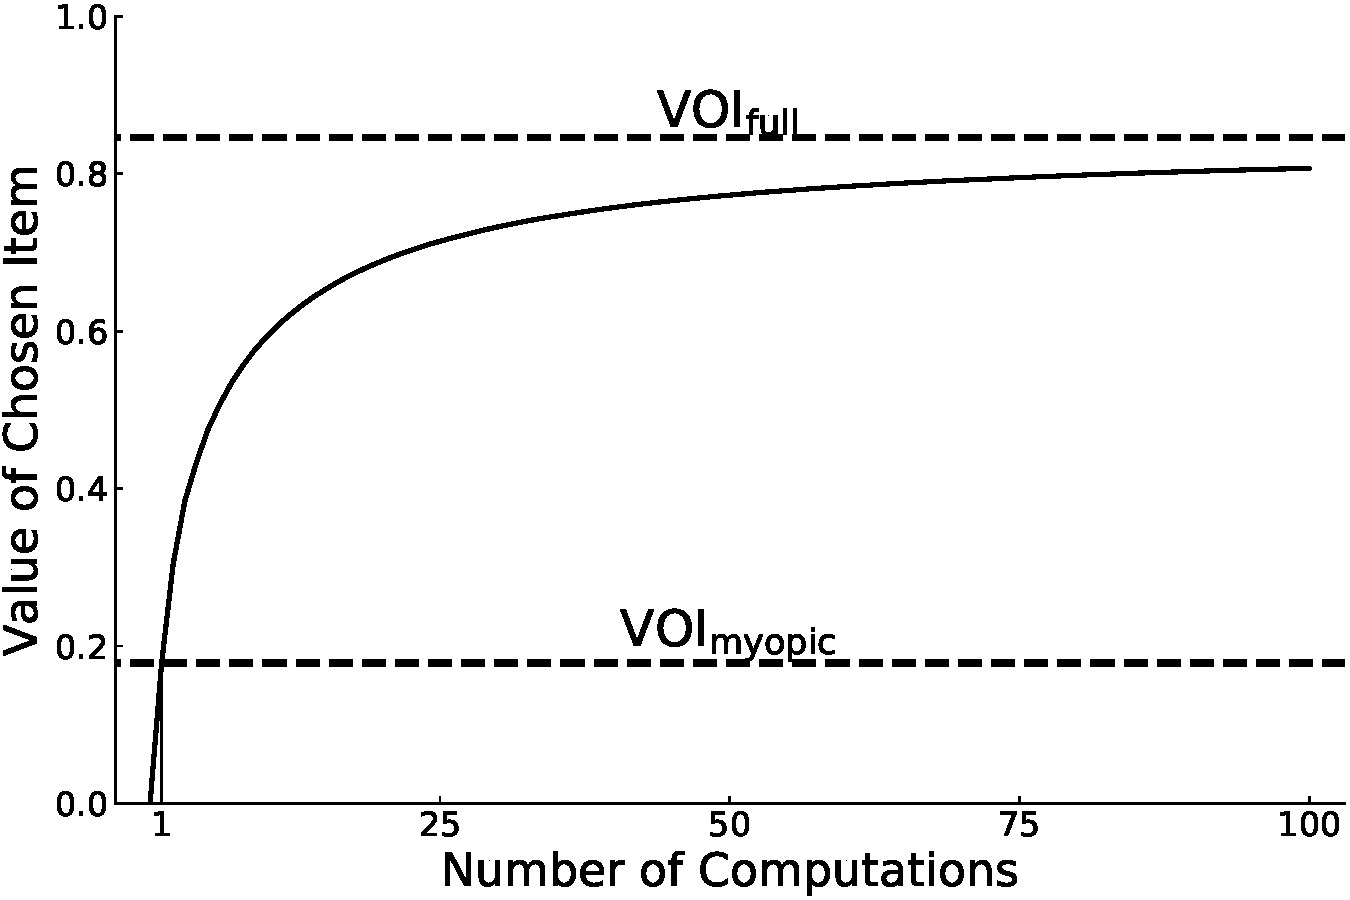
\includegraphics[width=0.7\textwidth]{figs/attention/supp-voi-vpi.pdf}
  \caption{\captiontitle{Illustration of the value of information features}.
    The solid line shows the average value of the item chosen after different numbers of computations selected by a near-optimal policy for the metalevel MDP defined in Section~\ref{sec:attention-mdp}, assuming no computational costs. The dashed lines show values for two of the VOI features in the initial belief state: $\VOImy$ is the value after one computation and $\VPI$ is the asymptotic value after infinite computations.
  }
  \label{fig:bmps-voi}
\end{figure}

\subsection{Bounding the value of information}

As illustrated in Figure \ref{fig:bmps-voi}, the value of information acquired by an optimal metalevel policy increases monotonically with the number of computations it performs. Moreover, it is bounded by two values, each giving the VOI associated with a distribution of possible beliefs.

The minimum VOI is the value of information produced by the first computation. In this case, the distribution of beliefs is simply $B' = T(b, c)$. Thus, the myopic value of information is defined as
\begin{equation*}
  \VOImy(b,c) =  \VOI(T(b, c)) = \expectunder{R(b', \bot)}{b' \sim T(b, c)}.
\end{equation*}

The maximum VOI is the value of full, or ``perfect'' information \citep{howard1966information}. In this case, each of the possible future beliefs assigns all probability to a single world state; denote such a belief as $b^*_w = \Uniform(\{w\})$.
% \footnote{%
%   For notational clarity, we assume countable world states. For continuous world states, $b^*_w$ takes the form of a Dirac delta.
% } 
The distribution over these beliefs, $B^*_b$ is defined $\Pr(B^*_b = b^*_w ) = b(w)$. Intuitively, the subjective probability of coming to the belief that assigns all probability to state $w$ is equal to the subjective probability that $w$ is in fact the true world state. We can then define the value of full information as
\begin{equation}
  \VPI(b) = \VOI(B^*_b) = \expectunder{R(b^*_w, \bot)}{w \sim b}
\end{equation}


\subsection{Learning to select computations}

Given that $\VOImy(b,c)$ and $\VPI(b)$ provide lower and upper bounds on the value of information, it follows that the true optimal value of information ($\VOI(B_N)$ in Equation~\ref{eq:Q-VOI}) is an interpolation between these two values. This suggests the following approximation,
\begin{equation}\label{eq:bmpsQ}
  Q\bmps(b, c; \vec{w}) = w_1 \VOImy(b,c) + w_2 \VPI(b) - (\cost(b, c) + w_\cost)
\end{equation}
where $w_1 + w_2 = 1$ are the interpolation weights and $w_\cost \geq 0$ captures the expected cost of future computations. In specific domains, we may be able to identify additional VOI features that quantify the value of acquiring intermediate amount of information. For example, in Chapter~\ref{sec:attention} we will use a VOI feature for learning the exact value of a single item in the choice set. One can add as many such terms as one likes, adding an additional weight for each, and ensuring that they all sum to one. Even with additional features, the approximation makes the very strong assumption that the interpolation weights and expected future cost are constant across belief states, an assumption that will almost certainly not hold. However, it turns out that this rough approximation is sufficient to produce near-optimal metalevel policies in some cases. This policy is defined as
\begin{equation}
  \pi\bmps(s; \vec{w}) = \Uniform\left(\argmax_a Q\bmps(s, a; \vec{w})\right).
\end{equation}

How should the weights be determined? Treating the approximation literally, the most appropriate strategy would be Q-learning, which tries to find weights that predict that actual returns of the policy. However, because the approximation is so rough, this turns out not to work well in practice. Instead, we can treat the weights as arbitrary parameters of a policy and use policy search to find weights that maximize performance. That is
\begin{equation}
  \vec{w}^* = \argmax_\vec{w} \expect{
    \sum_{t=1}^{\tmax} R(m_t, c_t, w)
  }{
    c_t \sim \pi\bmps(m_t; \vec{w})
  }
\end{equation}

The key advantage to BMPS over a more generic RL algorithm is that the policy has a very small number of parameters. This allows us to use an efficient search strategy such as Bayesian optimization. \citet{callaway2018learning} present an evaluation of BMPS trained with Bayesian optimization on several benchmark tasks, finding that it outperforms the blinkered policy described above as well as a generic DQN. In a cognitive modeling application, consistency may be more important than efficiency; in these cases, we can use exhaustive search algorithms that produce similar results when run multiple times. I describe such a method in Section~\ref{sec:attention-ucb}.

\section{Summary}

In this chapter, I introduced the formal framework of metalevel Markov decision processes. Below I briefly summarize the key points to take away from this section:

\begin{itemize}
  \item A Markov decision process (MDP) models a sequential decision problem with a set of states the environment can be in, a set of actions the agent can take, a transition function specifying how actions affect the environment state, and a reward function specifying the immediate utility gained by executing each action in each possible state (Section~\ref{sec:mdps}).

  \item A metalevel Markov MDP models the problem posed by an agent's internal cognitive environment. Here, states correspond to mental states, actions correspond to cognitive operations, the transition function specifies how operations update mental state, and the reward function specifies both cognitive cost and also the utility of the external action that is taken as a result of cognition. A metalevel MDP also includes a set of world states  that determines both the outcome of cognitive operations and also the utility of external actions. (Section~\ref{sec:metalevel-mdps}).

  \item The optimal policy for a metalevel MDP corresponds to an optimal cognitive process, an optimal strategy for selecting which cognitive operation to perform next given the current mental state (Section~\ref{sec:metamdp-policy}).

  \item We can adopt two views of computation: a mechanical view that treats mental states and actions as exactly analogous to external states and actions, and a Bayesian view that formalize computations as internal experiments that generate information about the world (Sections~\ref{sec:two-views} and~\ref{sec:bayesian-metamdp}). Adopting the latter view allows us to transform a metalevel MDP into an equivalent ``marginalized'' MDP (Section~\ref{sec:metamdp-marginalized}).

  \item Identifying optimal policies for metalevel MDPs can be challenging due to the very large state and action spaces (Section~\ref{sec:computing}). Adopting a combination of model-free and model-based techniques can be an effective way to solve this challenging problem (Section~\ref{sec:bmps}).
\end{itemize}

In the following three chapters, I show how my colleagues and I have applied this framework to characterize optimal cognitive processes for attention, memory, and planning. As we shall see, this will highlight many of the ways that human cognitive processes are well adapted to both our internal and external environments, revealing new insights about both how our minds work and why they work that way.

